% ===============================================
% MATH 373: Intro to Numerical Analysis           Fall 2021
% prog2_testing_template.tex
% June 8, 2021
% ===============================================

% -------------------------------------------------------------------------
% You can ignore this preamble. Go on
% down to the section that says "START HERE" 
% -------------------------------------------------------------------------

\documentclass{article}

% load packages
\usepackage{amsmath,amsfonts,graphicx,amsthm,amssymb,hyperref,xcolor}

% Define default environments
\newenvironment{theorem}[2][Theorem]{\begin{trivlist}
\item[\hskip \labelsep {\bfseries #1}\hskip \labelsep {\bfseries #2.}]}{\end{trivlist}}
\newenvironment{lemma}[2][Lemma]{\begin{trivlist}
\item[\hskip \labelsep {\bfseries #1}\hskip \labelsep {\bfseries #2.}]}{\end{trivlist}}
\newenvironment{claim}[2][Claim]{\begin{trivlist}
\item[\hskip \labelsep {\bfseries #1}\hskip \labelsep {\bfseries #2.}]}{\end{trivlist}}
\newenvironment{problem}[2][Problem]{\begin{trivlist}
\item[\hskip \labelsep {\bfseries #1}\hskip \labelsep {\bfseries #2.}]}{\end{trivlist}}
\newenvironment{proposition}[2][Proposition]{\begin{trivlist}
\item[\hskip \labelsep {\bfseries #1}\hskip \labelsep {\bfseries #2.}]}{\end{trivlist}}
\newenvironment{corollary}[2][Corollary]{\begin{trivlist}
\item[\hskip \labelsep {\bfseries #1}\hskip \labelsep {\bfseries #2.}]}{\end{trivlist}}

\newenvironment{solution}{\begin{proof}[Solution]}{\end{proof}}

%adjust to 1 in margins
  \addtolength{\oddsidemargin}{-.875in}
   \addtolength{\evensidemargin}{-.875in}
    \addtolength{\textwidth}{1.75in}

    \addtolength{\topmargin}{-.875in}
    \addtolength{\textheight}{1.75in}
    
% Define Shortcuts
\def\ds{\displaystyle}
\def\beginrefs{\begin{list}%
        {[\arabic{equation}]}{\usecounter{equation}
         \setlength{\leftmargin}{2.0truecm}\setlength{\labelsep}{0.4truecm}%
         \setlength{\labelwidth}{1.6truecm}}}
\def\endrefs{\end{list}}
\def\bibentry#1{\item[\hbox{[#1]}]}

\begin{document}



% ------------------------------------------ %
%                 START HERE             %
% ------------------------------------------ %

\large

{\Large Math 373, Introduction to Numerical Analysis}

\begin{center}
{\Large Author: \hfill Amanda Lauen} % Replace "Author's Name" with your name
\end{center}
\par \medskip \par
{\Large Programming Assignment: 2} 
\par \bigskip \par

% Complete summary and remove the instructions in red
{\bf Summary:} {\color{black} The assignment expresses to construct a program that uses the Secant Method to calculate the approximation of a function using two points.  The primary numerical method used to solve this problem was the use of the Secant Method to determine the approximation of a given function from the user between two points.  The Secant Method was described in section 2.4 in Tea Time Numerical Analysis [LB16].  This method was also described in lecture 5.1 of Dr. Kyle Riley’s notes [KR21]. It was discussed visually in the video lectures ‘Secant Method Derivation’ and ‘Secant Method Convergence’ given by Dr. Kyle Riley [KR21].} 
\par \bigskip \par

% Complete methods and remove the instructions in red
{\bf Methods:} {\color{black} 
The methods used in this program surrounded the ideas of the Secant Method described in class, in lecture videos, the notes, and in the textbook.  The possible outcomes of this mathematical problem are an approximation and a flag that indicates whether the program was executed correctly.  The first outcome is the approximation that is calculated within the code using the Secant Method.  The second outcome is a flag with a range of 0 to 3, each indicating specific success or error that the program encounters.  These two outputs are produced and printed in the command window when the code is running correctly.
\par \medskip
The code presents three flags to indicate if the output is acceptable or not.  If the flag is zero, then the output is fine and will run properly.  However, if the flag is one, then the inputs inputted are outside the given interval in the code.  The code determines if the tolerance is less than 0 or if a is equal to b, then the flag one is printed.  This line of code also helps in determining the convergence of the function.  If the flag is 2, then the algorithm fails to converge, which in simple terms means it diverges.  The final flag, introduced after acknowledgment from the September 29th in-class lecture, is flag 3.  If the flag is 3, then the xk value (b in this code) equals 0, which indicates a horizontal line.  According to Dr. Kyle Riley, “[The Secant M]ethod does require each secant line to be non-horizontal” [KR21].  The given function must be a non-horizontal line to get the proper answer for this problem.
\par \medskip
I made this program as efficient as possible by checking the error between iterations to ensure I got the correct error.  I have it commented out in my code, but I wanted to include this check to show how I was checking to ensure I was getting the correct outputs.  
\par \medskip
I believe it is possible to check that a solution to f(x)=0 exists for this code.  The way to do this is to choose the correct values that can help prove its existence.  I tested this on my code using a = 1, b = 2, and tol = 0.001, and I got a flag of 0 (meaning that it ran properly) and an approximation of 2.  By determining the correct points that can help identify its existence and hand calculating the answer as well, as I did for my program, I think it can help check if f(x)=0 has a solution. 
\par \medskip
I also believe that it is possible to verify that the calculated approximation is a feasible solution to the problem.  I believe that creating the proper check could help in seeing if the approximation is a feasible solution. I think that having a piece of the code that checks the actual roots and the real answer and comparing it to the approximation would be one of the ways to check to see if the approximation is a feasible solution.  Setting an acceptable error for it to be feasible can also help with this calculation like if it has less than 0.01 for an error, it is feasible.  This notion can be changed depending on what the user determines as the correct amount of error is acceptable for testing the feasibility of the approximation.

}
\par \bigskip \par


% Complete testing and analysis, please remove the instructions in red
{\bf Testing and Analysis:} {\color{black} I tested my program by first calculating the iterations and the error by hand to see the results and testing them on my program to see if they matched.  One example that I did was the function $x^2-4=0$.  I first graphed the function by hand and determined that the original roots of this function are x = -2 and x =2, so I knew that this was the given interval that my result needed to fall between.  I then chose the a and b values 1 and 4 as the coordinate pair (1,4) to determine the approximation.  I also gave the tolerance to be 0.001.  I then assigned a to be x\textsubscript{0} and b to be x\textsubscript{1} to match with the Secant Method variables.  Then, I calculated the first iteration and updated the a and b values to match the new x\textsubscript{1} and x\textsubscript{2} values.  I then calculated the error and created a chart that documented each iteration and the values that I received to determine the convergence.  This process by hand will be shown in more detail in the Appendix.  
\par \medskip
For the number of iterations that the code goes through to determine convergence, I chose 500.  I chose this number because if the algorithm performs more iterations than that number, the algorithm fails for that specific case.  Many reasons for the failure could that that the tolerance is extremely small, the limits are not correctly defined, etc.  Thus, this high number helps indicate whether a function truly does or does not converge.

}
\par \bigskip \par

%Hit list is optional, but is evidence of higher learning, developing strong skills in reviewing are extremely valuable. Please remove instructions in red.
{\bf Hit List: }{\color{black} The only problem with my code that I could not figure out is the output of flags 2 and 3.  I tried several points, functions, and tolerances to see if either of these would print out, but they did not.  It would be one of the things I would try and work on fixing if I had more time to work on this program.  I would have also liked to put more test cases for the function, a, b, and tolerance given by the user.  These tests would help check for situations where a user can put in something that would give an error or be deemed correct.  I think that if more checks were included, it could be one program that could handle any function, points, or tolerance.}
\par \bigskip \par

%Integrity Statement Leave the statement in red and follow it with ``I affirm that this program submission complies with the integrity specifications of this assignment. I understand if I am in violation of the integrity specification then I will get a zero on the assignment and receive an overall reduction in my course grade by one letter grade. ``

{\bf Academic Integrity}: {\color{black} The goal of this assignment is that everyone write their own code. This means you should not copy any code from any other source (the only exception are the templates provided by the instructor.) If you copy any code then you are in violation of integrity specifications of this assignment. If you provide your code to others then you are also in violation of the integrity rules of this assignment. 
\par \medskip
I affirm that this program submission complies with the integrity specifications of this assignment. I understand if I am in violation of the integrity specification then I will get a zero on the assignment and receive an overall reduction in my course grade by one letter grade .
}


% Add references here, list alphabetically according to last name of primary author.
\section*{References}
\beginrefs


\bibentry{LB16}{\sc Leon Brin},
{\it Tea Time Numerical Analysis (Experiences in Mathematics)  (2nd ed.)}, 2016. Website: \href{http://lqbrin.github.io/tea-time-numerical/}{lqbrin.github.io/tea-time-numerical} .
\bibentry{KR21} {\sc Kyle Riley}, Class Lecture, Math 373: Introduction to Numerical Analysis, Lecture, August 2021. 

\endrefs

\bigskip \par \bigskip
%%%------------------------------------------------------
%  Appendix, remove the red comments when completing this section. 
%%----------------------------------------------------------
{\Large {\bf Appendix}} \par \medskip

{\color{black}  	As stated in the Testing and Analysis portion of this report, I calculated example functions, points, and tolerances that could be entered into my program by hand and double-checked to see if they would correspond with the program I built.  The main example stated in the Testing and Analysis portion will be highlighted which was $f = x^2-4=0,$ a = 1, b = 4, and tol = 0.001.  I first assigned a and b to x\textsubscript{0} and x\textsubscript{1} to match with the notation in the Secant Method formula:
\par \medskip
x\textsubscript{0}=a=1
\par \medskip
x\textsubscript{1}=b=4
\par \medskip
	I then conducted the first iteration, x\textsubscript{2}, to be:
	\par \medskip
x\textsubscript{2}=4-f(4)(4-1)/(f(4)-f(1))=4-12(3)/15=1.6
\par \medskip
	I then updated the values of a and b with the x1 and x2 values calculated above:
	\par \medskip
a=x\textsubscript{1}=4
\par \medskip
b=x\textsubscript{2}=1.6
\par \medskip
	I then calculated the error of the first iteration and got:
	\par \medskip
$error=$$|b-a|$$/$$|a|$$=$$|1.6-4|$$/$$|4|$$=0.6$
\par \medskip
	I then hand calculated up to 5 iterations by hand which the values can be seen below in the chart.  Note that the values a\textsubscript{old}, b\textsubscript{old} refers to a and b before updating them (before calculating x\textsubscript{2}). At the same time, a\textsubscript{new}, b\textsubscript{new} are the values of a and b after updating them (after calculating x\textsubscript{2}).
} 
\begin{figure}[!ht]
\centering  %centering can be used to center the image
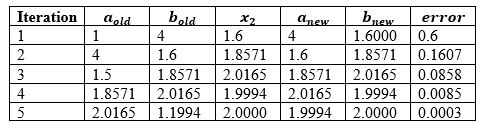
\includegraphics[height=35mm]{Programs/Program 2/Chart for Prog2.PNG}
 \caption{Results from Secant Method Example 1}
 \label{f:Chart}
\end{figure}
\par \medskip
{\color{black} Given the chart, the error of the fifth iteration is less than the tolerance given (0.0003 < 0.001), which means that the algorithm converged in 5 iterations.  Thus, the solution is that approximation is about 2.0000.  
\par \medskip
To prove that these calculations were correct, I ran the function $x^2-4$, a=1, b=4, and tol=0.001 through my code and got the following results:
\par \medskip
$f  = @(x) x^2-4;$
\par \medskip
a = 1;
\par \medskip
b = 4;
\par \medskip
tol = 0.001;
\par \medskip
[flag,approx]=prog2b820474(f,a,b,tol)
\par \medskip
flag =0
\par \medskip
approx = 1.9994
\par \medskip
I verified that the correct values were being run by defining them first in the command window for this code run.  As seen from the code above, the approximation given in the output is around two, so it concludes that the code and the worked out by hand method match.
\par \medskip
An example of the printing of the first flag is when I changed a and b values to equal each other:
\par \medskip
$f = @(x) x^2-4;$
\par \medskip
a=1;
\par \medskip
b=1;
\par \medskip
tol=0.001;
\par \medskip
[flag, approx] = prog2b820474(f,a,b,tol)
\par \medskip
flag = 1
\par \medskip
approx = -99
\par \medskip
I then tested my code with the following function, a, b, and tolerance values:
\par \medskip
Case 1:
\begin{itemize}
    \item f=log(x-1)+cos(x-1)
    \item a=1.4
    \item b=1.4048
    \item tol=0.001
\end{itemize}
\par \medskip
Case 2:
\begin{itemize}
    \item $f=x^2-9$
	\item a=-2
    \item b=-1
	\item tol=0.010
\end{itemize}
\par \medskip
Case 3:
\begin{itemize}
    \item $f=x^6-4x-3$
	\item a=-3
    \item b=-714
	\item tol=0.076
\end{itemize}
\par \medskip
These cases represent the cases in which the code can present the correct flags when needed and calculate the approximation efficiently given the values f, a, b, and tol.
\par \medskip
From the above example call functions, I concluded that:
\par \medskip
1. The approximations found by the function for the examples done by hand are the same.
\par \medskip
2.	When the input values are out of range, the algorithm fails to converge, or if the xk value is a horizontal line, it provides the desired results.
\par \medskip
3. When the input values are valid, the error function must be smaller than the given tolerance to be valid.
\par \medskip
Thus, the code and the calculations by hand prove that the program is producing accurate calculations.

}


% ---------------------------------------------------
% Anything after the \end{document} will be ignored by the typesetting.
% ----------------------------------------------------

\end{document}